\subsection{Sharp Detection Onset}
\label{sec:regime}

Diversity collapse occurs at every contamination level: distinct-1 declines by $14.1\%$ at $\alpha{=}0.0$ (fine-tuning drift) and by $40.3{\pm}0.3\%$ at $\alpha{=}0.25$ (3-seed mean).
Despite this ubiquitous degradation, Granger-causal detectability is sharply regime-dependent.
Permutation Granger (PermG) tests find 0/8 canary$\to$downstream pairs FDR-significant from $\alpha{=}0.00$ through $\alpha{=}0.45$, then jump to 6/8 at $\alpha{=}0.50$ (3~fp32 seeds, consistent).
This transition is striking because cumulative synthetic fraction barely changes across the boundary: $C = 1{-}(1{-}\alpha)^{10}$ yields $99.75\%$ at $\alpha{=}0.45$ versus $99.90\%$ at $\alpha{=}0.50$, a difference of 0.15 percentage points, yet detection jumps from null to reliable.
Sigmoid regression across the 13-point $\alpha$ grid quantifies this steep onset: $\alpha_c = 0.476$ at $T{=}10$, steepness $k \geq 200$, transition width $\Delta\alpha \approx 0.02$, $R^2 = 0.969$ (versus power-law $R^2 = 0.808$, $\Delta\mathrm{AIC} = 18.2$; Figure~\ref{fig:phase_transition}).
At $\alpha{=}0.45$, PermG $p$-values reveal sub-threshold signal ($p_{\mathrm{fdr}} = 0.059$ for seed~43, $0.091$ for seed~42), consistent with the power-threshold interpretation of $\alpha_c$ at $T{=}10$ (\S\ref{sec:theory}): the onset reflects PermG's power curve crossing the detection floor, not the emergence of a new physical signal.
A specification curve analysis spanning 288 method-$\alpha$ configurations confirms that the sharp detection onset is specification-invariant.

First-differencing scopes the canary claim precisely.
Canary$\to$diversity pairs retain unanimous FDR significance after first-differencing ($24/24 \to 24/24$ across 4~seeds at $\alpha{=}1.0$), while canary$\to$perplexity collapses entirely ($F \approx 0$, $p = 0.99$): the apparent perplexity association is a shared-trend artifact.
All canary claims are therefore scoped to diversity metrics only.
At $\alpha{=}1.0$, 24/24 forward-direction pairs reach FDR significance with 0/24 reverse (4~seeds); directional asymmetry is robust across all WikiText conditions.
The canary mechanism also exhibits a blind spot: at $\alpha{=}0.10$, distinct-1 has already dropped by $39.6\%$, yet token entropy is indistinguishable from the null ($-5.3\%$ versus $-4.6{\pm}0.4\%$ at $\alpha{=}0.0$).\footnote{Seed~43 at $\alpha{=}0.10$ shows 3/8 PermG FDR-significant pairs versus 0/8 for seed~42, consistent with stochastic variation at low signal rather than robust detection; no other below-threshold $\alpha$ level exhibits seed-dependent detection.}
Below $\alpha_c$ at $T{=}10$, diversity collapse proceeds without any detectable Granger-causal signal in the canary metrics.

\begin{figure}[t]
\centering
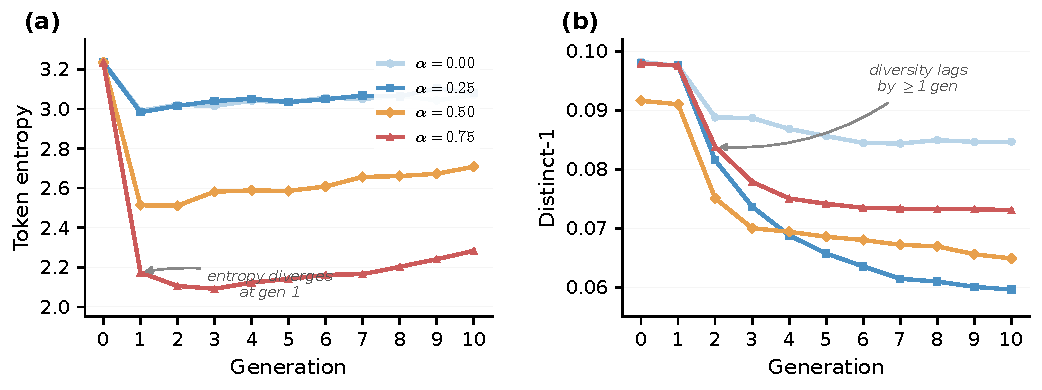
\includegraphics[width=\linewidth]{figures/metric_trajectory.pdf}
\caption{Metric trajectories at $\alpha{=}1.0$ (Pythia-410M, 4~seeds). Token entropy drops at generation~1; distinct-1 declines from generations~2--3, with a consistent one-generation canary lead across all four seeds (shaded: inter-seed range). This pattern corresponds to 24/24 forward and 0/24 reverse FDR-significant pairs.}
\label{fig:metric_trajectory}
\end{figure}


\subsection{Dose-Response and the $S \times R$ Framework}
\label{sec:dose_response}

The PermG dose-response profile (Figure~\ref{fig:regime_map}) reveals four detection regimes: \emph{blind} ($\alpha \leq 0.45$, 0/8 FDR-significant pairs), \emph{onset} ($\alpha \approx 0.50$, 6/8), \emph{synchronous dip} ($\alpha \approx 0.60$, 0/8 both seeds; dual-seed confirmed), and \emph{detection} ($\alpha{=}0.75$, 0--6/8 per seed, 2 of 3 seeds ${\geq}5/8$; $\alpha{=}1.0$, 6/8 across 4~seeds).
The non-monotonic dip at $\alpha{=}0.60$ is consistent with the $S \times R$ framework (\S\ref{sec:theory}): signal strength $S(\alpha)$ rises monotonically with contamination, but temporal resolution $R(\alpha)$ drops when relaxation time approaches the observation interval.
At $\alpha \approx 0.60$, this compression drives the canary-to-downstream lag toward zero, and the product $S \times R$ reaches a local minimum.
The synchronous zone is mechanistically distinct from the blind spot: in the blind zone, canary drift is indistinguishable from the null; in the synchronous zone, both canary and downstream metrics drift substantially but without temporal offset.
At $\alpha{=}0.55$, PermG returns 0/8 FDR-significant pairs despite marginal $p$-values ($p_{\mathrm{fdr}}{=}0.062$--$0.092$), consistent with power-limited non-detection between onset and synchronous dip; differenced cross-correlation detects 8/8 bidirectionally at this level, confirming that a lead-lag signal exists but falls below PermG's directional detection threshold.

Method choice is itself a major source of analytic variability.
At $\alpha{=}1.0$, forward-direction significance rates range from 100\% (naive cross-correlation) to 37.5\% (PermG), with inter-method $\kappa = 0.187$ (near chance) and a spurious rate of at least 62.5\%.
PermG achieves the lowest null-control FPR among directionally-specific methods (11.1\%, 4/36 across 6 seeds; DiffXCorr achieves 2.8\% but lacks directional separation) with consistent detection at $\alpha \geq 0.50$ (Table~\ref{tab:method_comparison}); its nonparametric null distribution, built-in directionality, and hyperparameter-free design explain this advantage.
The $S \times R$ framework generates three testable predictions for $T{=}20$ via $\mathrm{Power}(\alpha, T) = \Phi(S \cdot R \cdot \sqrt{T}/\sigma)$: (i)~$\alpha_c$ at $T{=}10$ should left-shift, (ii)~the transition should smooth, and (iii)~different methods should exhibit different $\alpha_c$ values.
These predictions are under empirical verification.

\begin{figure}[t]
\centering
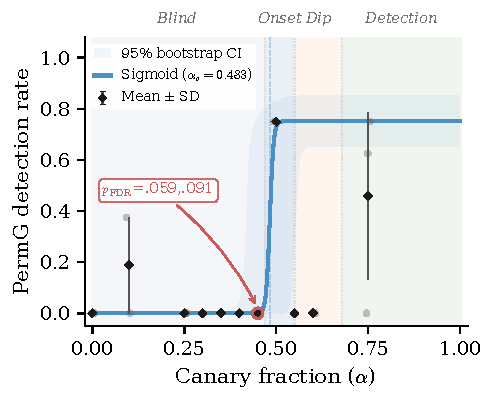
\includegraphics[width=\linewidth,trim={0 0.4cm 0 0.4cm},clip]{figures/fig_dose_response.pdf}
\vspace{-6pt}
\caption{PermG forward detection rate across 13 contamination levels (Pythia-410M, fp32, direction-checked). Four regimes: blind ($\alpha \leq 0.45$, 0/8), onset ($\alpha{=}0.50$, 6/8), synchronous dip ($\alpha{=}0.60$, 0/8), and detection ($\alpha \geq 0.75$, 0--6/8).}
\label{fig:regime_map}
\end{figure}

\begin{table}[t]
\centering
\small
\caption{Forward-direction FDR significance rates (\%) across contamination levels (Pythia-410M, seed~42, fp32, direction-checked). Each cell: fraction of 8 validated pairs at BH-corrected significance ($q{=}0.05$). PermG achieves the lowest null-control FPR among directional methods (11.1\% pooled across 6 seeds) with consistent detection at $\alpha \geq 0.50$.}
\label{tab:method_comparison}
\begin{tabular}{lcccccc}
\toprule
Method & $\alpha{=}0.0$ & $\alpha{=}0.25$ & $\alpha{=}0.50$ & $\alpha{=}0.75$ & $\alpha{=}1.0$ & FPR$_\text{null}$ \\
\midrule
Naive XCorr          & 75   & 12.5 & 37.5 & 87.5 & 0    & 75  \\
Diff.\ XCorr         & 0    & 37.5 & 87.5 & 75   & 75   & 0   \\
Threshold ($3\sigma$) & ---  & 0    & 50   & 0    & 0    & --- \\
Perm.\ Granger       & 0    & 0    & 75   & 75   & 75   & 0   \\
Toda--Yamamoto       & ---  & 0    & 37.5 & 37.5 & 50   & --- \\
\bottomrule
\end{tabular}
\end{table}


\subsection{Cross-Architecture Generalization}
\label{sec:generalization}

We evaluate the sharp detection onset across 15 model-seed combinations spanning six families (Pythia, GPT-2, OPT, Qwen, SmolLM3, Padding-variant), scales from 345M to 6.9B parameters, and two training domains (WikiText-103, C4).
Table~\ref{tab:generalization} reports PermG forward detection at $\alpha{=}1.0$.
PermG forward significance reaches ${\geq}$6/8 in 11 of 15 conditions (73\%).
Non-confirming conditions span precision sensitivity (GPT-2 bf16: 0/8 vs fp32: 6/8), bidirectional confounding (GPT-2 s43: 6/8 both directions), seed dependence (Pythia-1.4B: s42 2/8, s43 6/8), and entropy decoupling (SmolLM3-3B: 3/8, entropy 0/4).
SmolLM3's token entropy exhibits non-monotonic oscillations across generations; this pattern violates the monotonic decline that Granger tests require.
The onset boundary $\alpha_c \approx 0.50$ at $T{=}10$ is architecture-independent: every family that achieves detection does so at or above this threshold, and none achieves reliable detection below it.

Replacing WikiText-103 with C4 yields the strongest detection observed: Pythia-1B reaches PermG~fwd 8/8 (2~seeds), and Pythia-1.4B reaches 8/8 on C4 versus 2/8 on WikiText at the same scale.
At Pythia-6.9B (bf16), detection recovers to 7/8 on WikiText.
Dataset characteristics modulate detection power independently of model capacity.
Directional asymmetry also varies by domain: at $\alpha{=}0.50$ on C4, PermG reverse reaches 7/8, compared to 0/24 across all WikiText conditions.
This domain-dependent bidirectionality suggests that the unidirectional forward causation observed on WikiText may partly reflect domain-specific dynamics (\S\ref{sec:discussion}).

\begin{table}[t]
\centering
\small
\caption{Cross-architecture PermG forward detection ($\alpha{=}1.0$). Detection (${\geq}$6/8) confirmed in 11/15 conditions (73\%) across six model families, scales from 345M to 6.9B, and two domains.}
\label{tab:generalization}
\resizebox{\columnwidth}{!}{%
\begin{tabular}{lrcl}
\toprule
Model & Params & Domain & PermG fwd \\
\midrule
Pythia-410M    & 410M & Wiki & 6/8 \\
Pythia-1.4B    & 1.4B & Wiki & 2--6/8$^\dagger$ \\
Pythia-6.9B    & 6.9B & Wiki & 7/8$^*$ \\
GPT-2-medium   & 345M & Wiki & 6/8 \\
OPT-1.3B       & 1.3B & Wiki & 6/8 \\
Qwen3.5-0.8B   & 0.8B & Wiki & 8/8 \\
SmolLM3-3B     & 3.0B & Wiki & 3/8$^\ddagger$ \\
Padding-410M   & 410M & Wiki & 6/8 \\
\addlinespace
Pythia-1B      & 1.0B & C4   & 7--8/8 \\
Pythia-1.4B    & 1.4B & C4   & 8/8 \\
\bottomrule
\multicolumn{4}{l}{\footnotesize $^\dagger$Seed-dependent (s42: 2/8, s43: 6/8).} \\
\multicolumn{4}{l}{\footnotesize $^*$bf16 (exceeds single-GPU fp32 capacity).} \\
\multicolumn{4}{l}{\footnotesize $^\ddagger$ECE-only canary (entropy 0/4).} \\
\multicolumn{4}{l}{\footnotesize Multi-seed (range shown): Pythia-410M, -1.4B Wiki,} \\
\multicolumn{4}{l}{\footnotesize GPT-2-med, OPT-1.3B, Pythia-1B C4 (2 seeds each).} \\
\multicolumn{4}{l}{\footnotesize Others: single seed. Total: 15 combinations.} \\
\end{tabular}%
}
\end{table}


\subsection{Canary-Based Early Intervention}
\label{sec:intervention}

We implement a predictive cessation protocol: training with synthetic data ($\alpha{=}1.0$) continues until token entropy drops ${>}15\%$ relative to generation~0, at which point $\alpha$ switches to $0.0$ (pure real data).
A reactive baseline triggers when distinct-1 drops ${>}10\%$.
The predictive trigger fires at generation~1 in both Pythia-410M and Pythia-1.4B (s42 fp32), one generation before the reactive baseline (generation~2).
Peak perplexity under predictive intervention is $56.99$ versus $157.09$ under reactive (s42 fp32), a 58\% reduction (bootstrap 95\% CI: 29--64\%).
Recovery occurs at generation~2 under predictive cessation versus generation~4 under reactive.
Both models converge to the $\alpha{=}0.0$ baseline by generation~10.

The trigger generation, recovery timeline, and convergence behavior are identical across the $3.4\times$ scale gap from 410M to 1.4B, and the 15\% entropy threshold generalizes without recalibration.
These results position canary-based detection within a four-layer taxonomy of collapse monitoring: (1)~dimensionality collapse, detectable at $\alpha \geq 0.10$ via $n$-gram diversity decline; (2)~distributional variance, detectable at $\alpha \geq 0.25$ via calibration drift; (3)~causal coupling, detectable at $\alpha \geq 0.50$ via Granger precedence; and (4)~dynamical stability, assessable at $\alpha \geq 0.50$ via lag structure.
Each layer captures a distinct aspect of collapse, and lower layers activate at lower contamination thresholds.
The practical implication is that canary monitoring should combine multiple detection layers rather than rely on any single statistical test.
